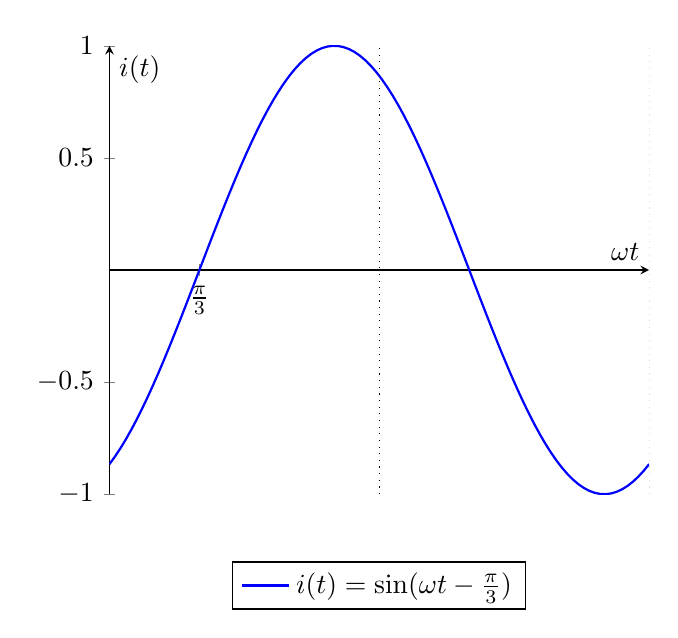
\begin{tikzpicture}

% Adjust the domain and samples according to your preference
\begin{axis}[
    xlabel={$\omega t$},
    ylabel={$i(t)$},
    domain=0:2*pi,
    samples=100,
    axis lines=middle,
    xtick={pi/3}, % Set x-axis tick at pi/3
    xticklabels={$\frac{\pi}{3}$}, % Label for the tick
    ytick={}, % Remove y-axis ticks
    legend style={at={(0.5,-0.15)},anchor=north},
]

% Plot the function
\addplot[blue,thick] {sin(deg(x - pi/3))};
\addlegendentry{$i(t) = \sin(\omega t - \frac{\pi}{3})$}

% Dotted vertical lines at x=pi and x=2pi
\draw[dotted] (axis cs:pi, \pgfkeysvalueof{/pgfplots/ymin}) -- (axis cs:pi, \pgfkeysvalueof{/pgfplots/ymax});
\draw[dotted] (axis cs:2*pi, \pgfkeysvalueof{/pgfplots/ymin}) -- (axis cs:2*pi, \pgfkeysvalueof{/pgfplots/ymax});

\end{axis}

\end{tikzpicture}
